\documentclass[11pt]{article}

\usepackage[portuguese]{babel}
\usepackage[utf8]{inputenc}
\usepackage{amsmath}
\usepackage{graphicx}
\usepackage{float}
\usepackage{subfig}
\usepackage{fixltx2e}
\usepackage{listings}
\usepackage[bottom]{footmisc}
\usepackage{color}
\usepackage{xargs}                      % Use more than one optional parameter in a new commands
\usepackage[pdftex,dvipsnames]{xcolor}  % Coloured text etc.
\usepackage[colorinlistoftodos,prependcaption,textsize=tiny]{todonotes}
\newcommandx{\unsure}[2][1=]{\todo[linecolor=red,backgroundcolor=red!25,bordercolor=red,#1]{#2}}
\newcommandx{\change}[2][1=]{\todo[linecolor=blue,backgroundcolor=blue!25,bordercolor=blue,#1]{#2}}
\newcommandx{\info}[2][1=]{\todo[linecolor=OliveGreen,backgroundcolor=OliveGreen!25,bordercolor=OliveGreen,#1]{#2}}
\newcommandx{\improvement}[2][1=]{\todo[linecolor=Plum,backgroundcolor=Plum!25,bordercolor=Plum,#1]{#2}}
\newcommandx{\thiswillnotshow}[2][1=]{\todo[disable,#1]{#2}}
\usepackage[font=footnotesize]{caption}

\definecolor{keywordcolor}{rgb}{0,0.4,0.7}
\definecolor{commentcolor}{rgb}{0.4,0.4,0.4} 	
\definecolor{mygray}{rgb}{0.5,0.5,0.5} 	% line counter color
\definecolor{mymauve}{rgb}{0.90,0.25,0.47}	% string color
\definecolor{codebackground}{rgb}{0.95,0.95,0.95} 

\lstset{ %
	backgroundcolor=\color{codebackground},   % choose the background color; you must add \usepackage{color} or \usepackage{xcolor}
	basicstyle=\ttfamily \footnotesize,        % the size of the fonts that are used for the code
	breakatwhitespace=false,         % sets if automatic breaks should only happen at whitespace
	breaklines=true,                 % sets automatic line breaking
	captionpos=b,                    % sets the caption-position to bottom
	commentstyle=\color{commentcolor},    % comment style
	deletekeywords={...},            % if you want to delete keywords from the given language
	escapeinside={\%*}{*)},          % if you want to add LaTeX within your code
	extendedchars=true,              % lets you use non-ASCII characters; for 8-bits encodings only, does not work with UTF-8
	keepspaces=true,                 % keeps spaces in text, useful for keeping indentation of code (possibly needs columns=flexible)
	keywordstyle=\color{keywordcolor},       % keyword style
	numbers=left,                    % where to put the line-numbers; possible values are (none, left, right)
	numbersep=5pt,                   % how far the line-numbers are from the code
	numberstyle=\tiny\color{mygray}, % the style that is used for the line-numbers
	rulecolor=\color{black},         % if not set, the frame-color may be changed on line-breaks within not-black text (e.g. comments (green here))
	showspaces=false,                % show spaces everywhere adding particular underscores; it overrides 'showstringspaces'
	showstringspaces=false,          % underline spaces within strings only
	showtabs=false,                  % show tabs within strings adding particular underscores
	stepnumber=1,                    % the step between two line-numbers. If it's 1, each line will be numbered
	%stringstyle=\color{mymauve},     % string literal style
	identifierstyle=\color{mymauve},
	tabsize=2                       % sets default tabsize to 2 spaces
}

\usepackage{titlesec}
\setcounter{secnumdepth}{4}
\titleformat{\paragraph}
{\normalfont\normalsize\bfseries}{\theparagraph}{1em}{}
\titlespacing*{\paragraph}
{0pt}{3.25ex plus 1ex minus .2ex}{1.5ex plus .2ex}

\numberwithin{equation}{section}

\linespread{1.3}
\usepackage{indentfirst}
\usepackage[top=2cm, bottom=2cm, right=2.2cm, left=2.2cm]{geometry}
\addto\captionsportuguese{\renewcommand{\contentsname}{Índice}}

\begin{document}

\begin{titlepage}
\begin{center}

\hfill \break
\hfill \break


\includegraphics[width=0.3\textwidth]{./logo}~\\[1cm]

\textsc{\LARGE Instituto Superior Técnico}\\[0.25cm]
\textsc{\Large Mestrado Integrado em Engenharia Electrotécnica e de Computadores}\\[1.8cm]
\textsc{\huge Arquitecturas Avançadas de Computadores}\\[0.25cm]

{\huge \bfseries Descrição do processador $\mu$Risc a funcionar em \textit{pipeline}\\[1.2cm]}

\begin{tabular}{ l l }
Guilherme Branco Teixeira & \hspace{2mm} n.º 70214 \\ 
Maria Margarida Dias dos Reis & \hspace{2mm} n.º 73099 \\
Nuno Miguel Rodrigues Machado & \hspace{2mm} n.º 74236 
\end{tabular}

\vfill

{\large Lisboa, 10 de Maio 2015} 

\end{center}
\end{titlepage}
 
\pagenumbering{gobble}
\clearpage

\tableofcontents
\pagebreak

\clearpage
\pagenumbering{arabic}

\section{Introdução}

Com este trabalho laboratorial pretende-se projectar um processador $\mu$Risc com funcionamento em \textit{pipeline}. O processador possui 4 andares de \textit{pipelining}: no primeiro andar é feito o \textit{instruction fetch} (IF), no segundo andar é feito o \textit{instruction decode} (ID) e o \textit{operand fetch} (OF), no terceiro andar são executadas operações da ALU (EX) e de acesso à memória de dados (MEM) e, por fim, no quarto é feita a escrita no banco de registos, o \textit{write back }(WB). Com o funcionamento em \textit{pipelining} podem ocorrer dois tipos de conflitos - de dados \textit{(data hazards)} e de controlo \textit{(control hazards)}. 

\section{Conflitos associados a uma arquitectura \textit{pipeline}}

\subsection{Conflitos estruturais}

Um conflito estrutural é quando a estrutura de um processador não tem os recursos suficientes para executar uma sequência de instruções em \textit{pipelining}. No entanto, o processador projectado não irá ter conflitos estruturais, isto porque terá recursos suficientes para executar todos os andares em \textit{pipelinig}.

\subsection{Conflitos de dados}

Um conflito de dados ocorre quando o \textit{pipelinig} muda a ordem de acesso a processos de escrita/leitura de operandos alterando a ordem pretendida das escritas e leituras dos registos.

Quando se fala em conflitos de dados fala-se de três tipos distintos:

\vspace{-1.5mm}

\begin{itemize}
	\item \textit{Read After Write} (RAW): ocorre quando uma instrução precisa de ler um valor que ainda não foi escrito na memória, pois pertence a uma instrução anterior que ainda não escreveu no seu registo de destino;
	\vspace{-2.5mm}
	\item \textit{Write After Read} (WAR): ocorre quando uma instrução necessita de escrever num registo, numa altura em que a instrução anterior ainda não leu o valor desse registo e necessita;
	\vspace{-2.5mm}
	\item \textit{Write After Write} (WAW): ocorre quando duas operações necessitam de escrever no mesmo registo ao mesmo tempo ou numa ordem incorrecta;
\end{itemize}

\vspace{-1.5mm}

No processador $\mu$Risc a projectar apenas ocorrem conflitos do tipo RAW. De facto, os conflitos do tipo WAR e do tipo WAW não ocorrem no processador a projectar, pois não existe qualquer tipo de \textit{bypassing} entre os seus andares, mantendo-se sempre a ordem das instruções intacta.

\subsection{Conflitos de controlo}

Quando uma instrução de controlo condicional é executada, esta tem duas possibilidades - ou altera o valor de PC (\textit{program counter}) para a próxima instrução (salto \textit{not taken}) ou para onde a instrução pretendida (salto \textit{taken}). 

\section{Métodos de resolução de conflitos}

\subsection{Conflitos de dados}

\begin{itemize}
	\item Solução 1: bloqueio dos andares do \textit{pipeline}, \textit{stall}, até que os dados correctos estejam disponíveis;
	\vspace{-2.5mm}
	\item Solução 2: se o dado correcto existir algures no \textit{pipeline}, estabelece-se um \textit{bypass} para o andar correcto, aplicando a técnica de \textit{forwarding};
	\vspace{-2.5mm}
	\item Solução 3: escalonar/reordenar as instruções - se a ordenação for feita pelo compilador tem-se um escalonamento estático e se for feita por \textit{hardware} é um escalonamento dinâmico;
\end{itemize}

\vspace{-1.5mm}

Analisando as soluções apresentadas verificou-se que o escalonamento estático e dinâmico não é a solução desejada devido a complexidade para um processador de 4 andares comparativamente às soluções expostas anteriores. 

Ponderou-se inicialmente a utilização de \textit{stalls} devido à facilidade de implementação mas, devido ao inconveniente de reduzir o número médio de instruções por ciclo (IPC), optou-se pela segunda solução que permite aumentar o valor de IPC com a contrapartida de ter uma maior complexidade de implementação.

\subsection{Conflitos de controlo}

\begin{itemize}
	\item Solução 1: \textit{Branch Target Buffer} (BTB) que é uma tabela que contém informação sobre os saltos já executados com o objectivo de tentar prever se uma nova instrução de salto é \textit{taken} ou \textit{not-taken}. A previsão é realizada por uma \textit{Branch Predict Buffer} (BPB), que é composta por 1 ou 2 \textit{bits}, e, caso a predição esteja correcta, diminui o número de \textit{stalls} necessários e, por sua vez, o número de ciclos de execução do programa;
	\vspace{-2.5mm}
	\item Solução 2: \textit{forwarding} de \textit{flags}, ou seja, lógica adicional que permite verificar se a previsão feita anteriormente pela BTB está correcta ou não, consoante a condição de salto;
	\vspace{-2.5mm}
\end{itemize}

Em análise às duas soluções apresentadas foi decidido que ambas seriam usadas no processador. Em relação à BTB, decidiu-se usar uma BPB de 1 \textit{bit}, pois não se achou necessário prever saltos com a profundidade de \textit{strong taken} e \textit{strong not-taken}.

De referir que, ao acrescentar \textit{forwarding} de \textit{flags}, o processador fica mais complexo mas, para verificar se a previsão foi efectuada correctamente, não é necessário aguardar dois ciclos mas sim apenas um, o que compensa para o valor de IPC.

\section{Estrutura do processador}

Como foi referido anteriormente, os conflitos de dados são resolvidos por \textit{forwarding} de dados e os conflitos de controlo são resolvidos por BTB e \textit{forwarding} de flags. De seguida, estão representados os circuitos e sinais que representam as unidades de resolução de conflitos.

\subsection{Circuitos e sinais na resolução de conflitos de dados}

A solução desejada é a aplicação de \textit{forwarding} de dados e este divide-se em duas partes: detecção de conflitos de dados e encaminhamento do resultado pretendido no andar que gera o conflito.

Nas figuras seguintes apresenta-se a lógica responsável para a detecção dos conflitos de dados.

\begin{figure}[H]
	\centering
	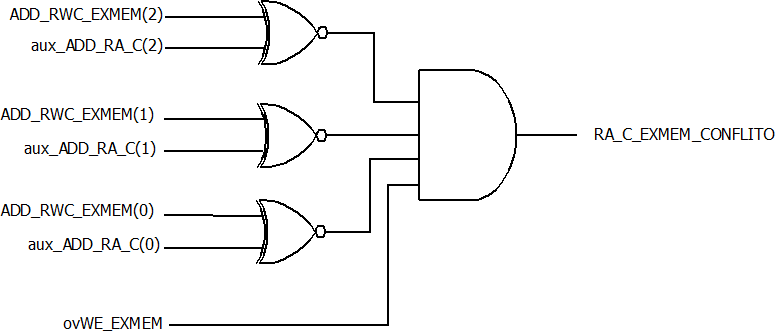
\includegraphics[keepaspectratio=true, scale=0.27]{imagens/DetecaodeconflitoEXMEM}
	\vspace{-0.5em}
	\caption{Detecção dos conflitos de dados para o operando A, no andar de EX/MEM.}
	\vspace{-0.8em}
\end{figure} 

Este circuito anterior representa a detecção de conflito de dados referente ao andar EX/MEM e consiste em comparar o endereço de escrita com o endereço do registo pretendido. Se estes forem iguais, o sinal \texttt{RA\_C\_EXMEM\_CONFLITO} tem valor lógico a 1 se o registo pretendido for o operando A ou o sinal \texttt{RB\_EXMEM\_CONFLITO}, que segue uma lógica equivalente à anterior, tem valor lógico a 1 se o registo pretendido for o operando B.

O circuito seguinte verifica se a instrução não é dependente de registos, para o registo A. É o caso de uma instrução de \textit{load} de constantes em que a constante a ser guardada pode, erradamente, endereçar um registo em que o valor pode estar no \textit{pipeline}. 

\begin{figure}[H]
	\centering
	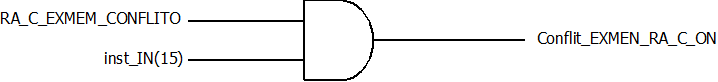
\includegraphics[keepaspectratio=true, scale=0.27]{imagens/DetecaodeconflitoEXMEM2}
	\vspace{-0.5em}
	\caption{Detecção dos conflitos de dados para o operando B, no andar de EX/MEM.}
	\vspace{-0.8em}
\end{figure} 

O circuito seguinte tem o mesmo objectivo que o circuito anterior mas para o registo B, pois existem instruções de salto que utilizam o registo B para efectuar os saltos relativos, como é o caso das instruções \textit{jump-and-link} e \textit{jump register}. Obtém-se assim dois sinais - um referente ao registo B, \texttt{Conflit\_EXMEM\_RB\_ON} e outro referente ao registo A, \texttt{Conflit\_EXMEM\_RA\_C\_ON}.
\begin{figure}[H]
	\centering
	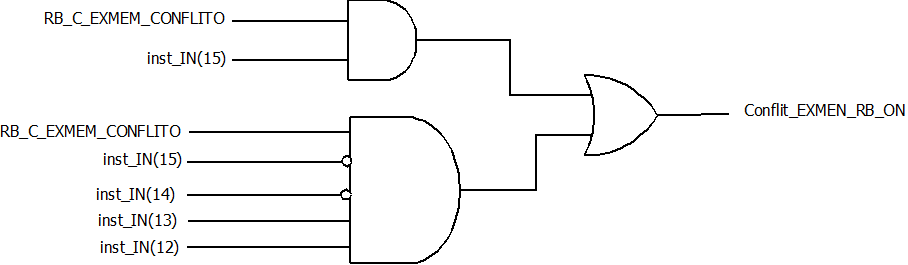
\includegraphics[keepaspectratio=true, scale=0.27]{imagens/DetecaodeconflitoEXMEMRB}
	\vspace{-0.5em}
	\caption{Circuito que permite verificar se uma instrução está associada à leitura de registos.}
	\vspace{-0.8em}
\end{figure} 

O circuito seguinte representa a detecção de conflito de dados referente ao andar WB, \textit{forwarding} que é necessário pois o banco de registo é síncrono. Como na situação anterior consiste em verificar o endereço de escrita com o endereço do registo pretendido e, se estes forem iguais, o sinal \texttt{RA\_C\_WB\_CONFLITO} tem sinal lógico a 1 se o registo pretendido for o operando A ou o sinal \texttt{RB\_WB\_CONFLITO} tem sinal lógico a 1 se o registo pretendido for o operando B.

\begin{figure}[H]
	\centering
	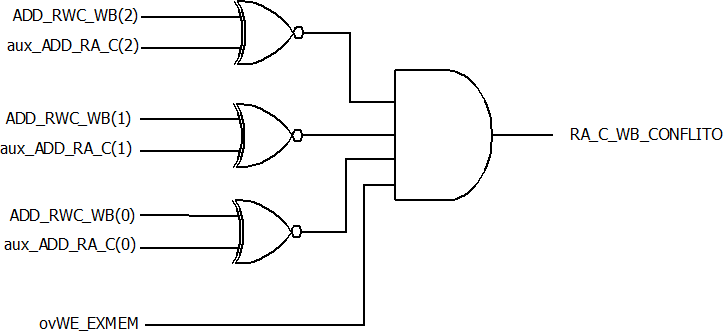
\includegraphics[keepaspectratio=true, scale=0.27]{imagens/DetecaodeconflitoWB}
	\vspace{-0.5em}
	\caption{Circuito que permite verificar se uma instrução está associada à leitura de registos.}
	\vspace{-0.8em}
\end{figure} 

Relativamente à detecção no andar de WB também é aplicado o circuito da Figura 2 para a detecção dos conflitos com registo A e o circuito Figura 3 para os conflitos com o registo B. Obtém-se assim dois sinais, um referente ao registo B, \texttt{Conflit\_WB\_RB\_ON} e outro referente ao registo A, \texttt{Conflit\_WB\_RA\_C\_ON}.

Geram-se assim dois sinais de controlo que seleccionam os valores dos operandos A e B - o sinal \texttt{mux\_RA} é um sinal de 2 \textit{bits} que consiste na concatenação do sinal \texttt{Conflit\_WB\_RA\_C\_ON} com \texttt{Conflit\_EXMEM\_RA\_C\_ON}, e o sinal \texttt{mux\_RB} é um sinal de 2 \textit{bits} que consiste na concatenação do sinal \texttt{Conflit\_WB\_RB\_ON} com \texttt{Conflit\_EXMEM\_RB\_ON}.

De seguida está representado o esquema geral de \textit{forwarding} nos andares de \textit{pipelining}.

\begin{figure}[H]
	\centering
	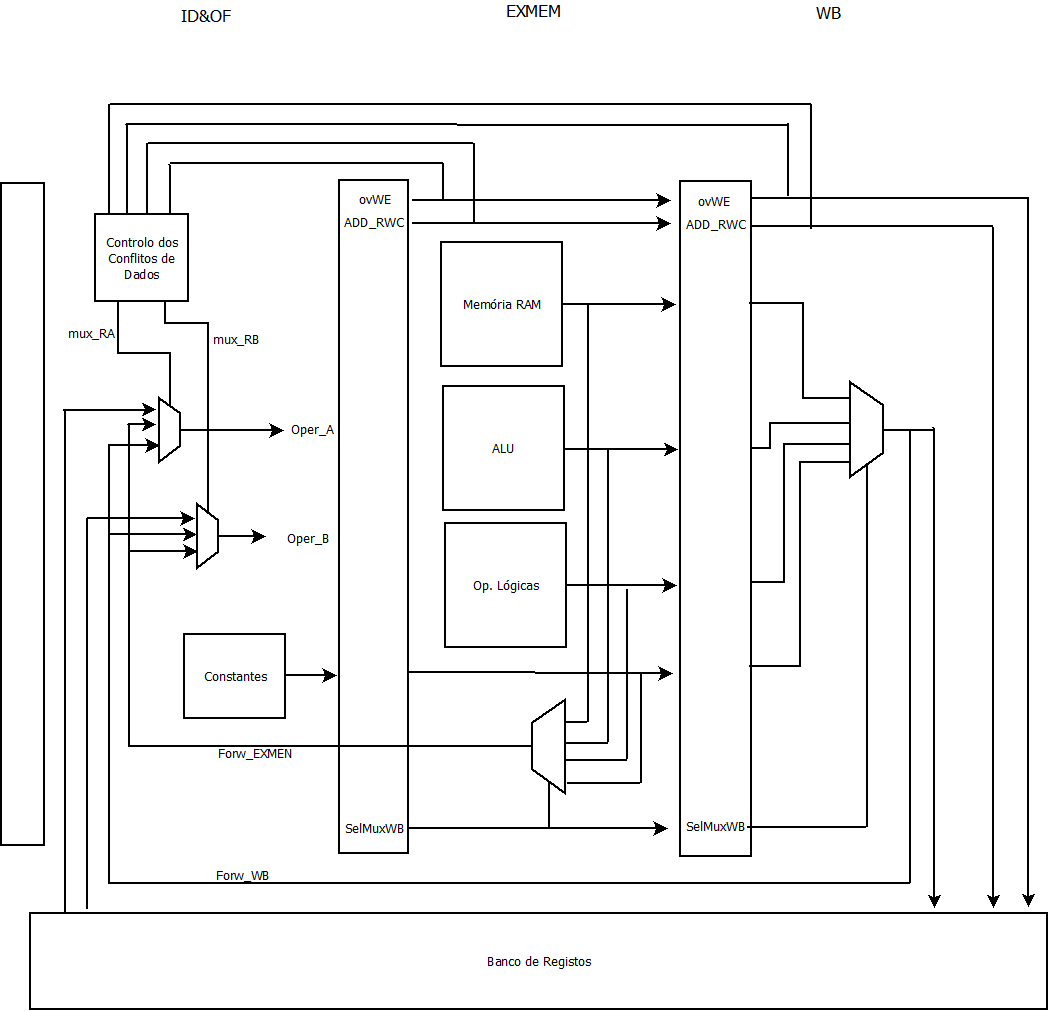
\includegraphics[keepaspectratio=true, scale=0.27]{imagens/DetecaodeconflitoGeral}
	\vspace{-0.5em}
	\caption{Esquema geral de resolução de conflitos de dados.}
	\vspace{-0.8em}
\end{figure} 

É de referir que foi acrescentado um MUX no andar EX/MEM de forma a obter o valor correcto do registo de escrita.

\subsection{Circuitos e sinais na resolução de conflitos de controlo}

Os circuitos e sinais para a resolução de conflitos de controlo são compostos por \textit{forwarding} de \textit{flags} e a criação de uma BTB. Estes circuitos e sinais estão divididos pelo andar IF e ID/OF.

No andar IF está implementado a tabela BTB. Esta tabela tem um tamanho de 512 posições, 9 \textit{bits} de endereçamento, e palavras de 16 \textit{bits} - 3 \textit{bits} de \textit{tag}, 12 \textit{bits} para o valor do salto, um \textit{bit} de predição e um \textit{bit} de validação.

A leitura da BTB é endereçada com os 9 \textit{bits} menos significativos do sinal \texttt{reg\_pc\_IN}, o valor do \textit{program counter}, originando quatro sinais - \texttt{MSB\_BTB}, \texttt{Jump\_From\_BTB},\texttt{Prediction\_Bit} e \texttt{Validate\_Bit}. estes sinais constituem o controlo de conflitos de controlo do andar IF, como se pode ver na imagem seguinte.

\begin{figure}[H]
	\centering
	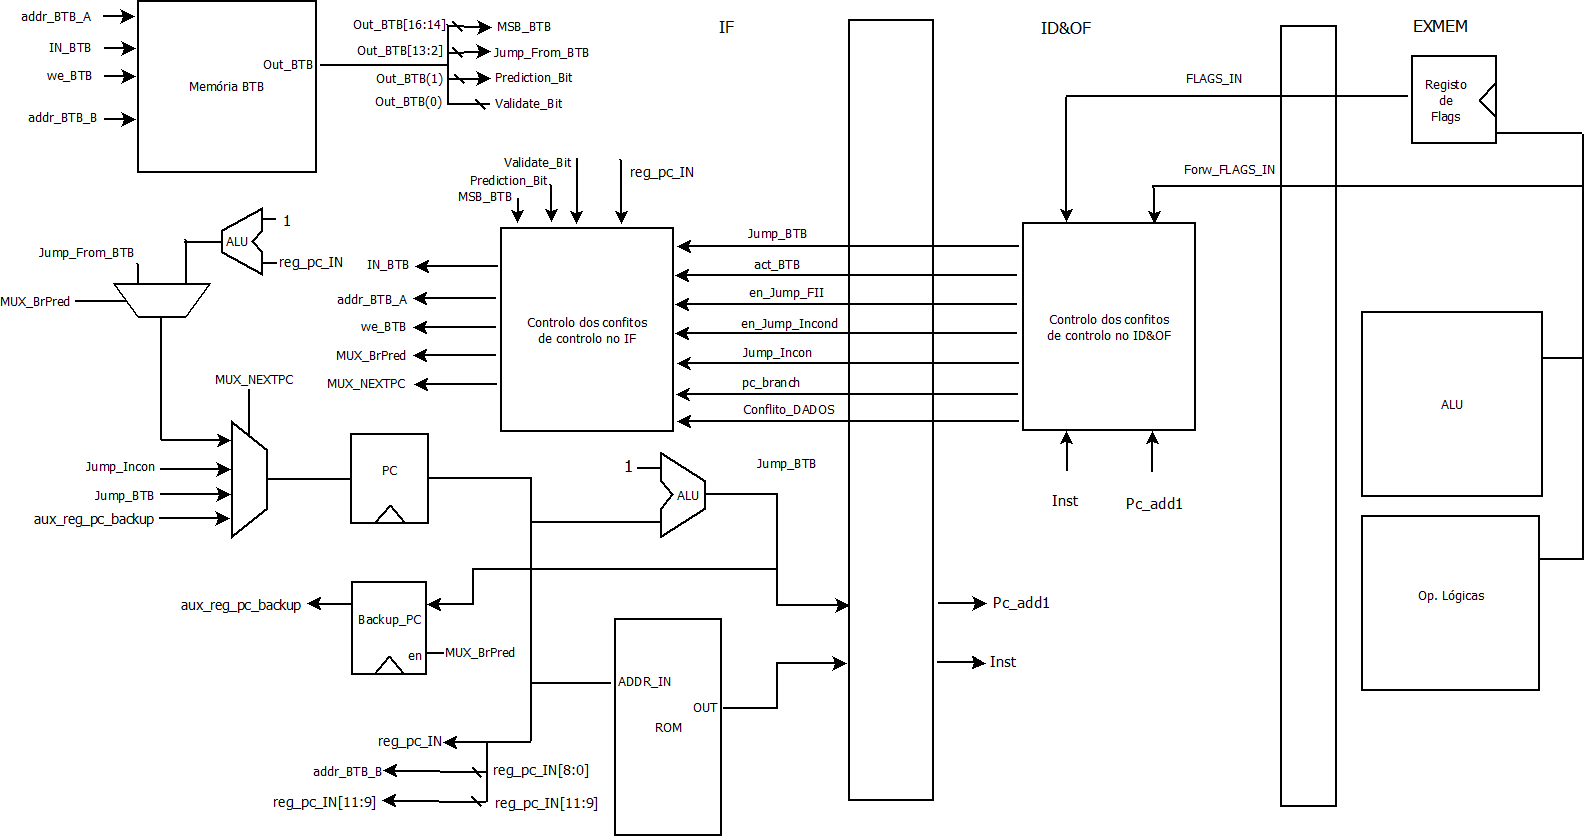
\includegraphics[keepaspectratio=true, scale=0.27]{imagens/ConflitodeContrologeral}
	\vspace{-0.5em}
	\caption{Esquema geral de resolução de conflitos de dados.}
	\vspace{-0.8em}
\end{figure}

Ao analisar o esquema anterior, defini-se dois sinais de controlo importantes na selecção do PC, \texttt{MUX\_BrPred} e \texttt{MUX\_NEXTPC}. 

O sinal \texttt{MUX\_BrPred} seleciona se o novo valor do PC é o sinal de salto da BTB ou PC + 1. Este sinal é gerado verificando se a \textit{tag} lida na BTB é igual aos 3 bits mais significativos do PC. Se for igual, o sinal \texttt{MUX\_BrPred} fica com o mesmo valor lógico do \textit{bit} de predição da BTB, \texttt{Prediction\_Bit}. De seguida está representado o esquema do sinal \texttt{Prediction\_Bit}:

\begin{figure}[H]
	\centering
	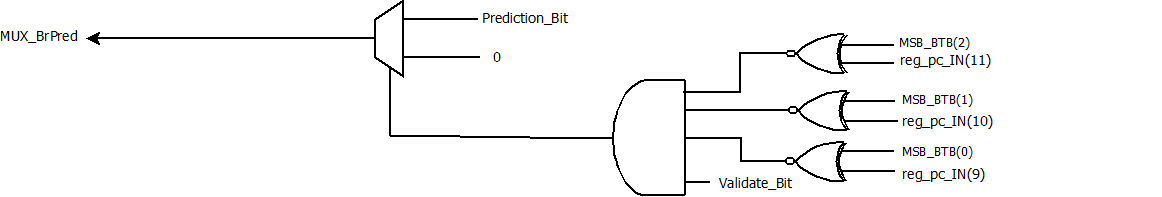
\includegraphics[keepaspectratio=true, scale=0.27]{imagens/Muxbrprd}
	\vspace{-0.5em}
	\caption{Esquema geral de resolução de conflitos de dados.}
	\vspace{-0.8em}
\end{figure}

O sinal \texttt{MUX\_NEXTPC} tem a função de seleccionar o PC a ser endereçado na ROM, existe 4 possibilidades, o PC gerado pelo sinal de controlo anterior, ou o salto condicional proveniente do andar ID/OF \texttt{Jump\_BTB}, ou o salto incondicional proveniente do andar ID/OF \texttt{Jump\_Incond}, ou o PC de \textit{backup}. De seguida está implementado a lógica do sinal  \texttt{MUX\_NEXTPC}.

\begin{figure}[H]
	\centering
	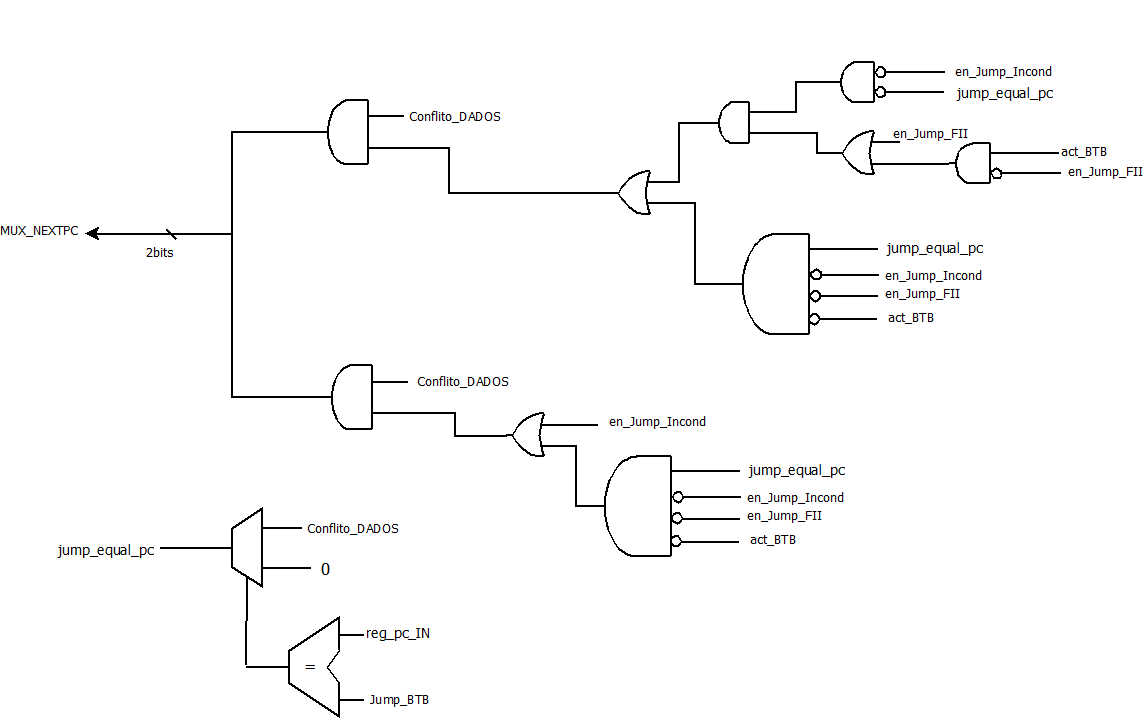
\includegraphics[keepaspectratio=true, scale=0.27]{imagens/MuxNEXTPC}
	\vspace{-0.5em}
	\caption{Esquema geral de resolução de conflitos de dados.}
	\vspace{-0.8em}
\end{figure}

\section{Testes de \textit{performance}}

Após o projecto do processador estar concluído procede-se à fase de testes. As métricas utilizadas foram: a frequência obtida com base no caminho crítico, o número de ciclos de execução até que o programa corra por completo, o tempo de execucão e o número de predicções falhadas por parte da BTB. Na tabela seguinte encontram-se os resultados obtidos para os três testes fornecidos.

\begin{table}[H]
	\centering
	\caption{\textit{Performance} obtida para os diversos testes com o processador demonstrado na aula.}
	\vspace{-1.5mm}
	\includegraphics[keepaspectratio=true, scale=0.40]{tabelas/processadororiginal}
	\label{tab:processadororiginal}
\end{table}

De referir que o caminho crítico do processador passa pelo circuito responsável pelo \textit{forwarding} de \textit{flags}, como se pode ver na próxima imagem.

\begin{figure}[H]
	\centering
	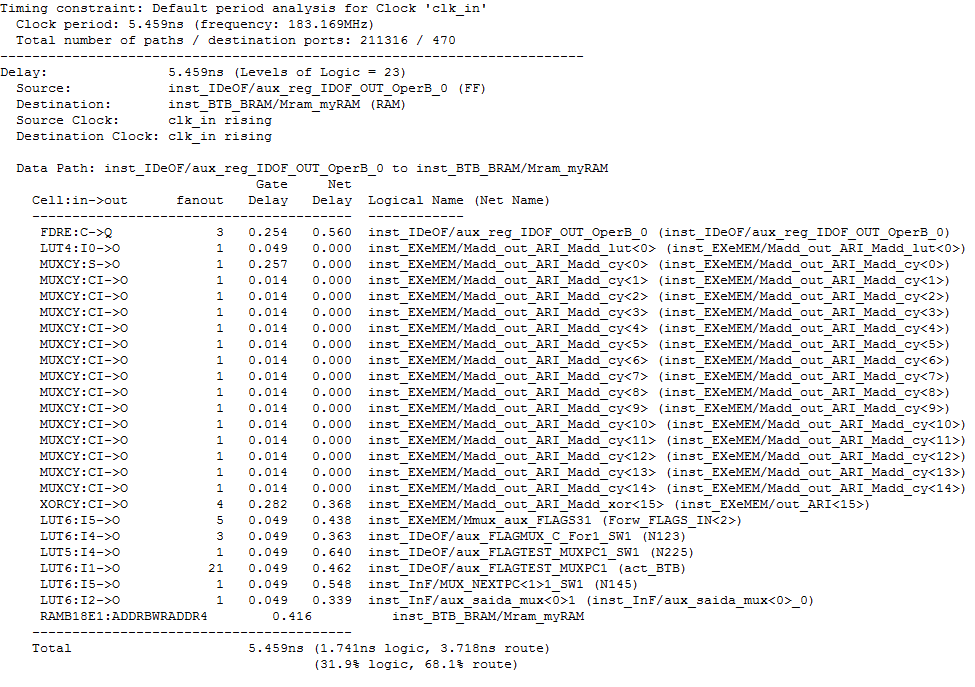
\includegraphics[keepaspectratio=true, scale=0.35]{imagens/freq183}
	\vspace{-0.5em}
	\caption{Caminho crítico do processador com frequência de 183,169 MHz.}
	\label{fig:183}
	\vspace{-0.8em}
\end{figure} 

No entanto, já após a demonstração do processador na aula laboratorial e depois de uma análise mais cuidada do caminho crítico concluiu-se que ainda era possível efecutar uma melhoria na \textit{performance} do $\mu$Risc. De facto, no caminho crítico existe um somador no andar de ID que pode passar para o andar anterior, ou seja, o andar de IF, o que permite aumentar a frequência do processador. 

Desta maneira, o novo caminho crítico permite ter uma frequência de 211,338 MHz. Na figura seguinte apresenta-se o novo caminho crítico como gerado pela ferramenta.

\begin{figure}[H]
	\centering
	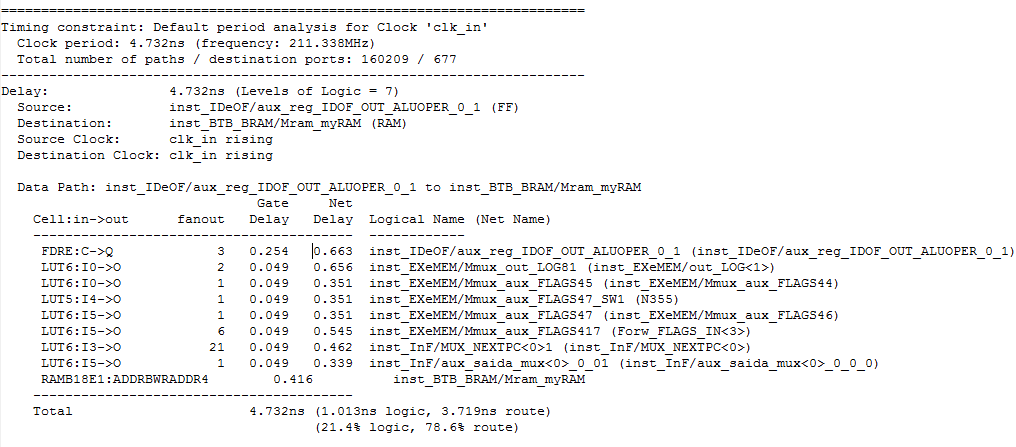
\includegraphics[keepaspectratio=true, scale=0.35]{imagens/freq211}
	\vspace{-0.5em}
	\caption{Caminho crítico do processador com frequência de 211,338 MHz.}
	\label{fig:211}
	\vspace{-0.8em}
\end{figure} 

Para se perceber melhor a influência que os métodos utilizados para resolver os conflitos têm no desempenho do processador foram realizados vários testes com diversas topologias do mesmo processador. Assim, fez-se testes para o processador falado anteriormente (processador \#1) e outros três processadores diferentes, cada um com diferentes combinações de métodos usados para corrigir os conflitos de dados e controlo, tal como se pode observar na Tabela \ref{tab:processadores}.

\begin{table}[H]
	\centering
	\caption{Diversas topologias do processador que foram testadas.}
	\vspace{-1.5mm}
	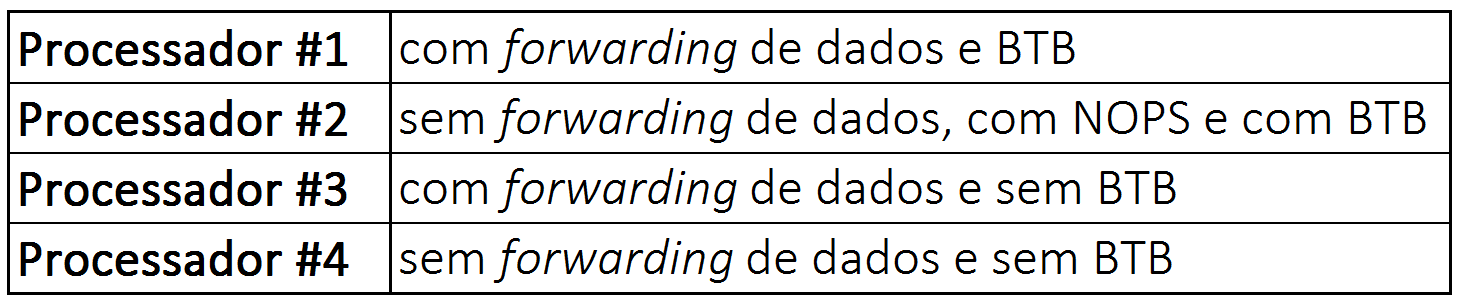
\includegraphics[keepaspectratio=true, scale=0.40]{tabelas/processadores}
	\label{tab:processadores}
\end{table}

O processador \#1 tem o caminho crítico da Figura \ref{fig:211}, assim como o processador \#2. Os processadores \#3 e \#4 tem o caminho crítico da figura apresentada de seguida.

\begin{figure}[H]
	\centering
	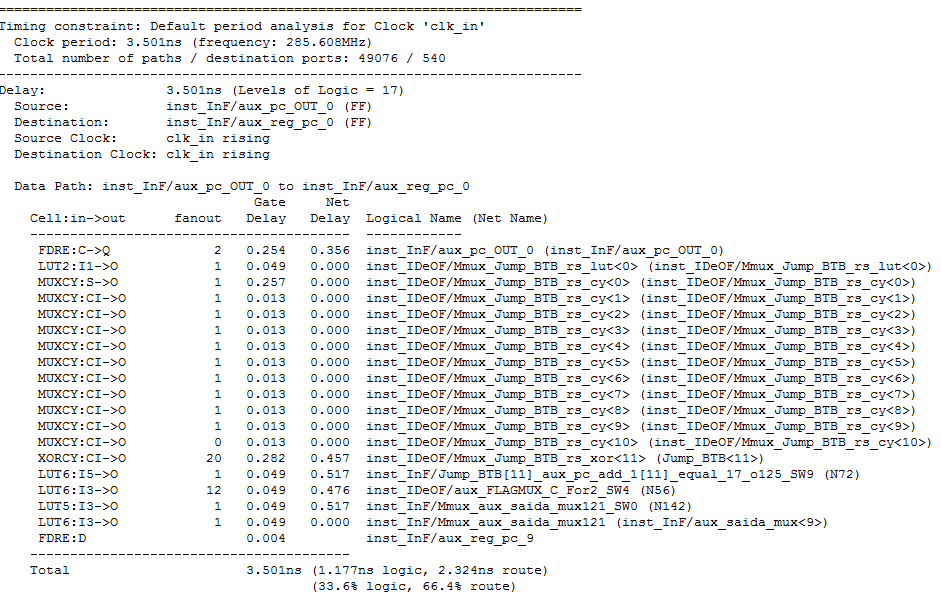
\includegraphics[keepaspectratio=true, scale=0.35]{imagens/freq285}
	\vspace{-0.5em}
	\caption{Caminho crítico do processador com frequência de 285,608 MHz.}
	\label{fig:285}
	\vspace{-0.8em}
\end{figure} 

Nas tabelas seguintes apresentam-se as métricas obtidas para os vários processadores para os três testes fornecidos.

\begin{table}[H]
	\centering
	\caption{Resultados obtidos para o teste$\#$1.}
	\vspace{-1.5mm}
	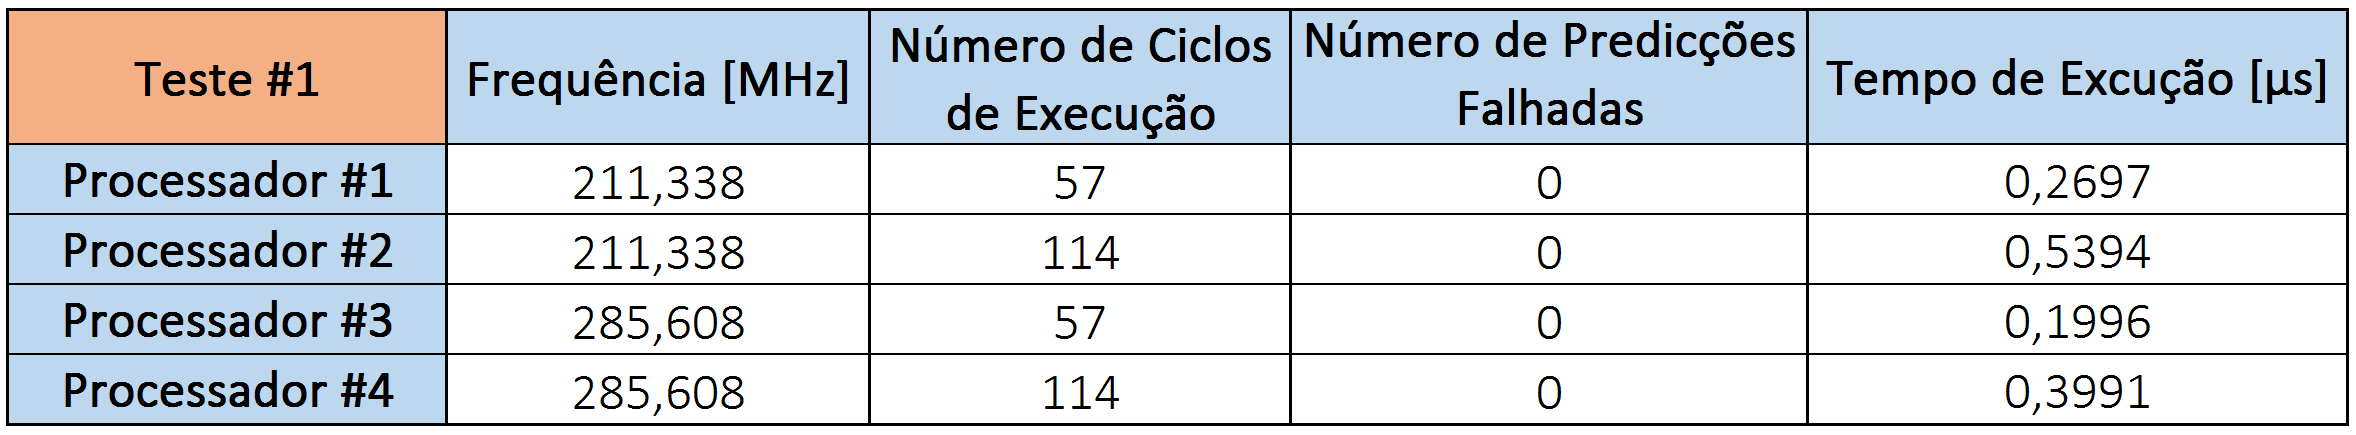
\includegraphics[keepaspectratio=true, scale=0.40]{tabelas/teste1}
	\label{tab:teste1}
\end{table}

\begin{table}[H]
	\centering
	\caption{Resultados obtidos para o teste$\#$2.}
	\vspace{-1.5mm}
	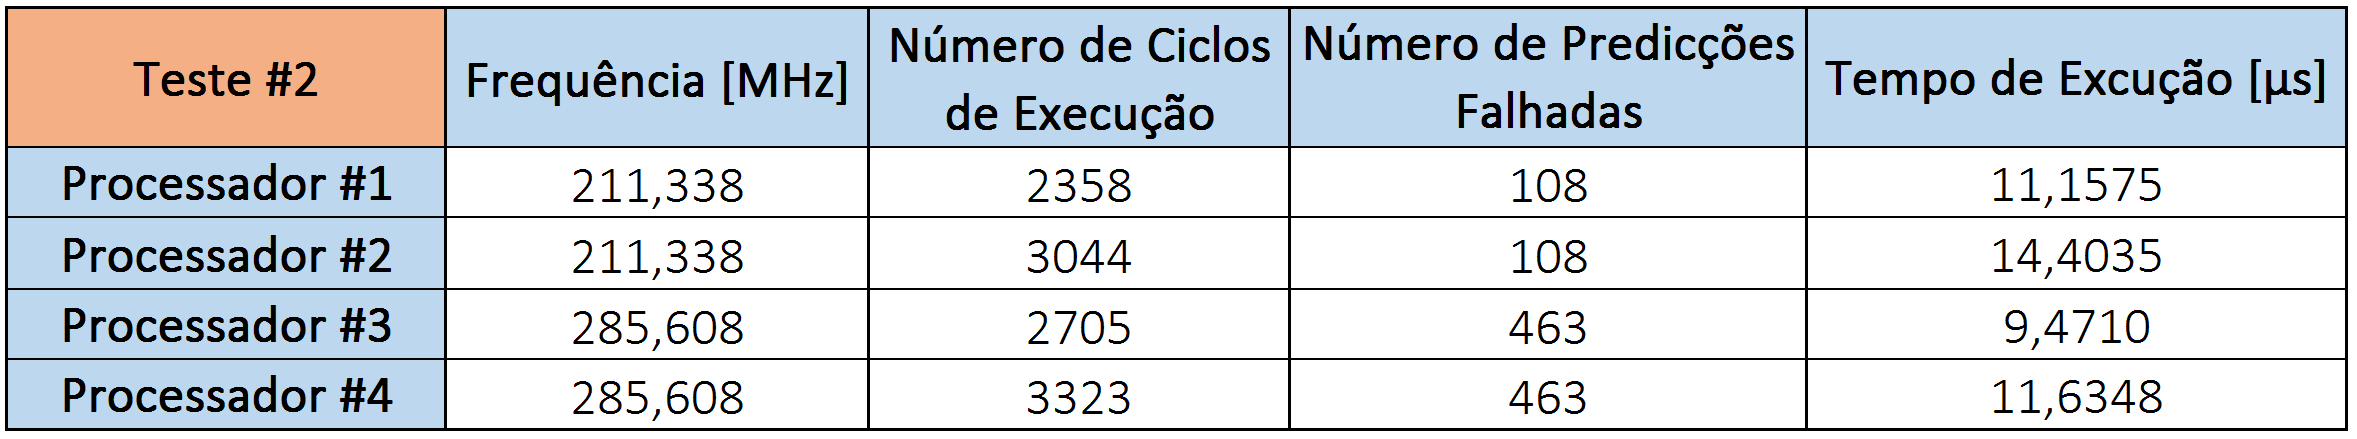
\includegraphics[keepaspectratio=true, scale=0.40]{tabelas/teste2}
	\label{tab:teste2}
\end{table}

\begin{table}[H]
	\centering
	\caption{Resultados obtidos para o teste$\#$3.}
	\vspace{-1.5mm}
	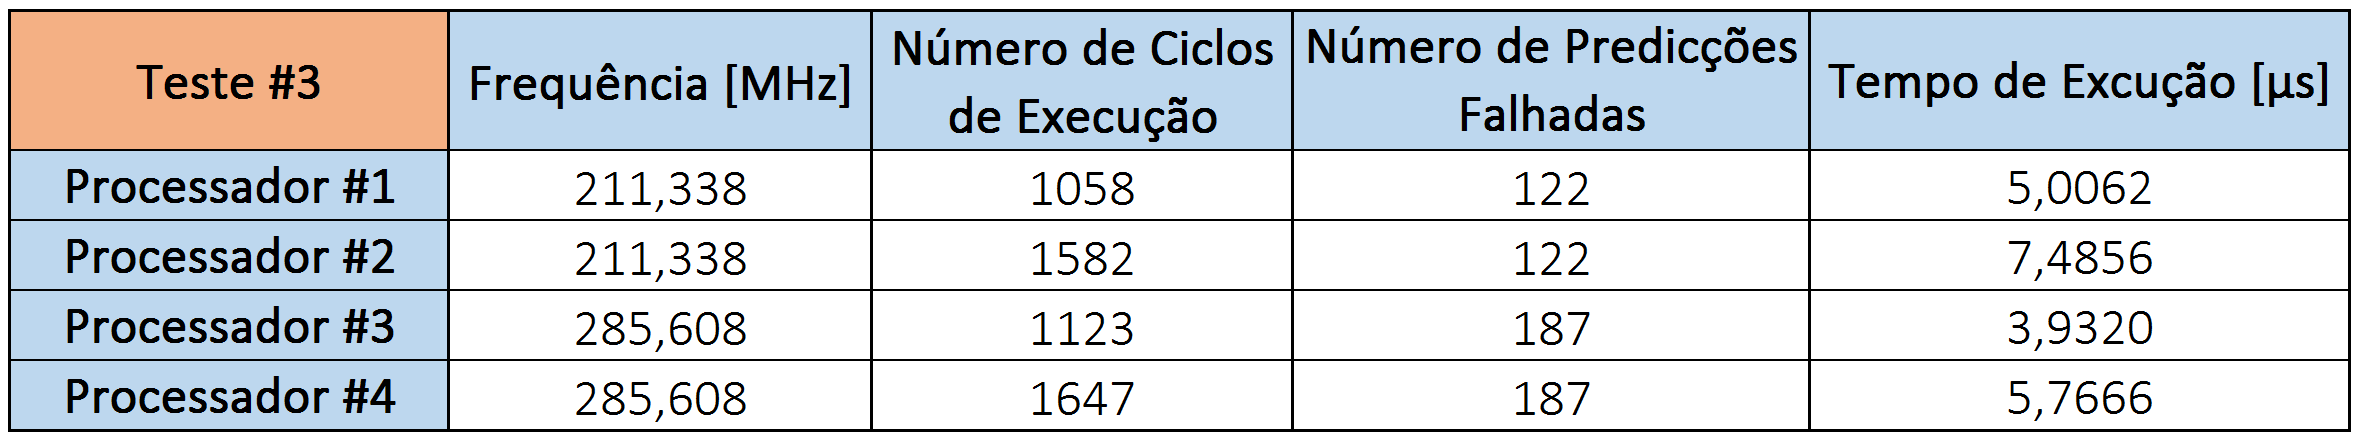
\includegraphics[keepaspectratio=true, scale=0.40]{tabelas/teste3}
	\label{tab:teste3}
\end{table}

Em análise aos resultados dos três testes realizados (Tabelas \ref{tab:teste1}, \ref{tab:teste2} e \ref{tab:teste3}), foi possível tirar as seguintes conclusões em relação ao \textit{forwarding} de dados e à BTB.

\subsection{Efeitos de \textit{forwarding} de dados}

Ao observar as características dos quatro processadores, percebe-se que é comparando os resultados entre os processadores \#1 e \#2 e também entre os processadores \#3 e \#4 que se consegue avaliar os efeitos de usar \textit{forwarding} de dados. Os cálculos do \textit{speed-up} são feitos através da equação \ref{eq:speed-up}.

\vspace{-3mm}
\begin{equation}
\text{\textit{speed-up}} = \frac{N_{\text{ciclos\textsubscript{processador\#2}}}}{N_{\text{ciclos\textsubscript{processador\#1}}}} = \frac{N_{\text{ciclos\textsubscript{processador\#4}}}}{N_{\text{ciclos\textsubscript{processador\#3}}}}
\label{eq:speed-up}
\end{equation}

\vspace{1mm}
Em relação ao primeiro teste (Tabela \ref{tab:teste1}), foi possível estabelecer um \textit{speed-up} de exactamente 2. Em relação ao segundo teste (Tabela \ref{tab:teste2}) os \textit{speed-up}'s alcançados foram de 1,291 e de 1,228, enquanto que no terceiro teste (Tabela \ref{tab:teste2}) foram alcançados \textit{speed-up}'s de 1,495 e de 1,467. Como nos três testes, tal como esperado, utilizar o método de \textit{forwarding de dados} influenciou a frequência dos processadores, podemos admitir que este método obtém resultados muito positivos.

\subsection{Efeitos de \textit{branch prediction}}

Ao observar as características dos quatro processadores, percebemos que é comparando os resultados entre os processadores \#1 e \#3 e também entre os processadores \#2 e \#4 que conseguimos avaliar os efeitos de usar uma BTB.

No primeiro teste (Tabela \ref{tab:teste1}) foi possível observar que nem sempre é positivo ter uma BTB, pois esta aumenta o tempo do caminho crítico, diminuindo assim a frequência do processador, e caso o teste não tenha saltos, o que se observa é um \textit{speed-up} menor que 1.

Em relação ao segundo teste (Tabela \ref{tab:teste2}), foi possível verificar que um processador com uma BTB, embora mais lento, apenas falhou apenas 23,3\% das predições, e que no terceiro teste falhou 65,2\% das predições. No caso destes dois testes, este aumento de precisão não correspondeu a um tempo de execução menor, no entanto, caso o teste fosse mais extenso seria possível observar um tempo de execução menor para um processador com \textit{branch prediction}.
\section{Conclusões}

Em primeiro lugar foi necessário colocar o circuito a funcionar em \textit{pipelining}, no entanto, no primeiro trabalho o circuito não estava a trabalhar em multi-ciclo, funcionava com todos os andares num só ciclo, este facto tornou a tarefa de colocar o circuito a funcionar em \textit{pipelining} mais complicada.
A identificação de quais os conflitos de dados e controlo a considerar foi uma tarefa relativamente simples comparada com a implementação da resolução desses conflitos. A maior dificuldade deste trabalho foi a implementação de umas das soluções para os conflitos de controlo, nomeadamente a BTB.

De referir que embora em testes tenham-se obtido resultados mais favorecedores (em termos de tempo de execução) para outros processadores sem a BTB, foi decidido que em testes mais exigentes(e com mais instruções de salto), um processador com BTB obteria resultados melhores, decidindo assim manter a BTB no processador final.

\pagebreak

\section{Anexos}

Em anexo ao relatório encontra-se o código VHDL que implementa o processador em regime de \textit{pipeline}.

\pagebreak

\listoftodos

\end{document}